\documentclass{beamer}
\bibliographystyle{amsalpha}
\usepackage{cite}
\usepackage[normalem]{ulem}
\usepackage{fancybox}
\usepackage{enumitem}
\setitemize{label=\usebeamerfont*{itemize item}
\usebeamercolor[fg]{itemize item}
  \usebeamertemplate{itemize item}}
\setbeamertemplate{footline}[frame number]{}
\setbeamertemplate{navigation symbols}{}
\graphicspath{{figures/}}

\title{The Heterogeneous Multiscale Method}
\subtitle{Combining Molecular Dynamics with Kinetic Theory}
\author[Price and Shohet]{Jake Price and Gil Shohet}
\institute[CPSSW]{Computational Physics Student Summer Workshop}
\date{\today}

\begin{document}
	\begin{frame}
		\titlepage
	\end{frame}
	
%	\begin{frame}[t]{Outline}
%		\tableofcontents
%	\end{frame}
	
	
	\section{Multiscale Overview}
	\subsection{Overview}
	
	\begin{frame}[t]{What is multiscale?}
	\vspace{0.25cm}
	\hfill
			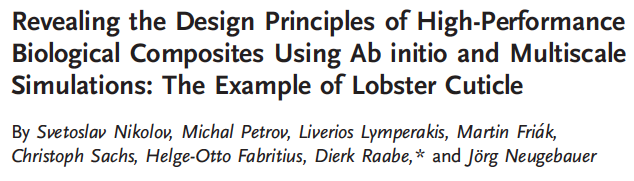
\includegraphics[width=\textwidth]{lobster.png}
			\hspace*{\fill}
			\vspace{1em}
			
				\hfill
			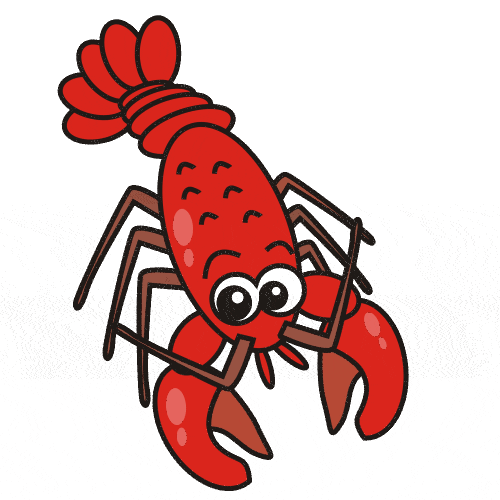
\includegraphics[width=0.3\textwidth]{lobsterclipart.png}
			\hspace*{\fill}
				\end{frame}
	
	\begin{frame}[t]{What is multiscale?}
			\em``[Multiscale methods] include analytical and numerical techniques that exploit the disparity of scales, as well as multi-physics problems...What we have in mind are problems that involve physical laws at different levels of detail, such as quantum mechanics and continuum models.''\\
		\normalfont\hfill-Weinan E \\
		\vspace{0.5cm}
		\begin{itemize}
			\item  Many phenomena have features with disparate length and times scales
			\vspace{0.3em}
			\item  Fully resolving these features is prohibitively expensive
			\vspace{0.3em}
			\item  Multiscale modeling allows us to resolve features of interest where they are important, and use a simpler model elsewhere
		\end{itemize}
	\end{frame}
	
	\subsection{Examples}
	\begin{frame}[t]{Multiscale Examples}
		\begin{columns}[T]
			\begin{column}{0.6\textwidth}
				\begin{itemize}
					\item  Adaptive Mesh Refinement (AMR)
					\vspace{8em}
					\item  Atmospheric Modeling
				\end{itemize}
			\end{column}
			
			\begin{column}{0.5\textwidth}
				\begin{center}
					\vspace{-1em}
					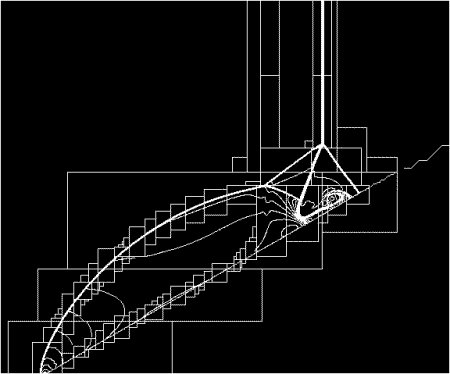
\includegraphics[width=0.8\textwidth]{Amrgridimg.jpg}
					\\\tiny AMR on shock impacting incline. (wikipedia.org)
				\end{center}
				\vspace{-1.5em}\hspace{-1.cm}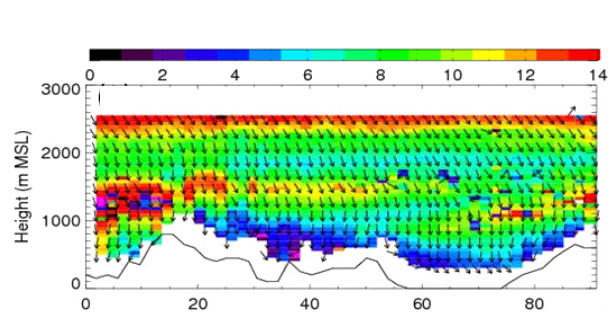
\includegraphics[width=1.1\textwidth]{atmospheric.png}
				\centering\\\tiny Atmospheric turbulence. (De Wekker, 2011)
			\end{column}
		\end{columns}
	\end{frame}
	
	\begin{frame}[t]{Multiscale Examples}
		\begin{columns}[T]
			\begin{column}{0.5\textwidth}
				\begin{itemize}
					\item  Multiphase Materials
					\vspace{7.5em}
					\item  Multi-physics Hierarchy
				\end{itemize}
			\end{column}
			
			\begin{column}{0.6\textwidth}
				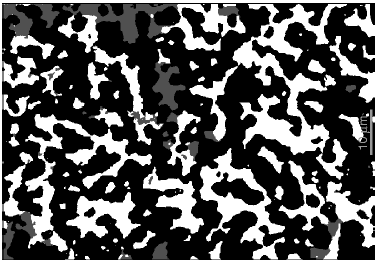
\includegraphics[width=0.7\textwidth]{multiphase.png}
				\centering\\\tiny Two-phase composite material. (Weinan E, 2011)\\
				\vspace{0.25em}\hspace{-1cm}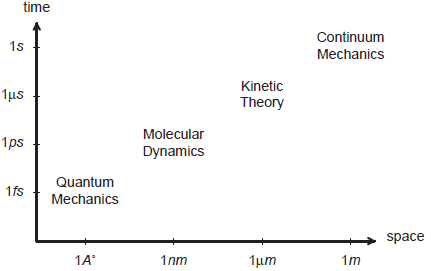
\includegraphics[width=1\textwidth]{hierarchy.png}
				\centering\\\tiny Multi-physics model hierarchy. (Weinan E, 2011)\\
			\end{column}
		\end{columns}
	\end{frame}
	
	\section{Heterogeneous Multiscale Method (HMM)}
	\subsection{Overview}
	\begin{frame}{What is the Heterogeneous Multiscale Method (HMM)?}
		\vspace{1em}
		\em``HMM is a framework for linking models at different scales. It follows a top-down strategy: The basic starting point is an incomplete macroscale model, with the microscale model used as a supplement. It consists of two main components: The macroscale solver and a procedure for estimating the missing numerical data from the microscale model."\hfill\\\hfill\normalfont -Weinan E, et al, 2006
		\vspace{-1em}
		\begin{center}
			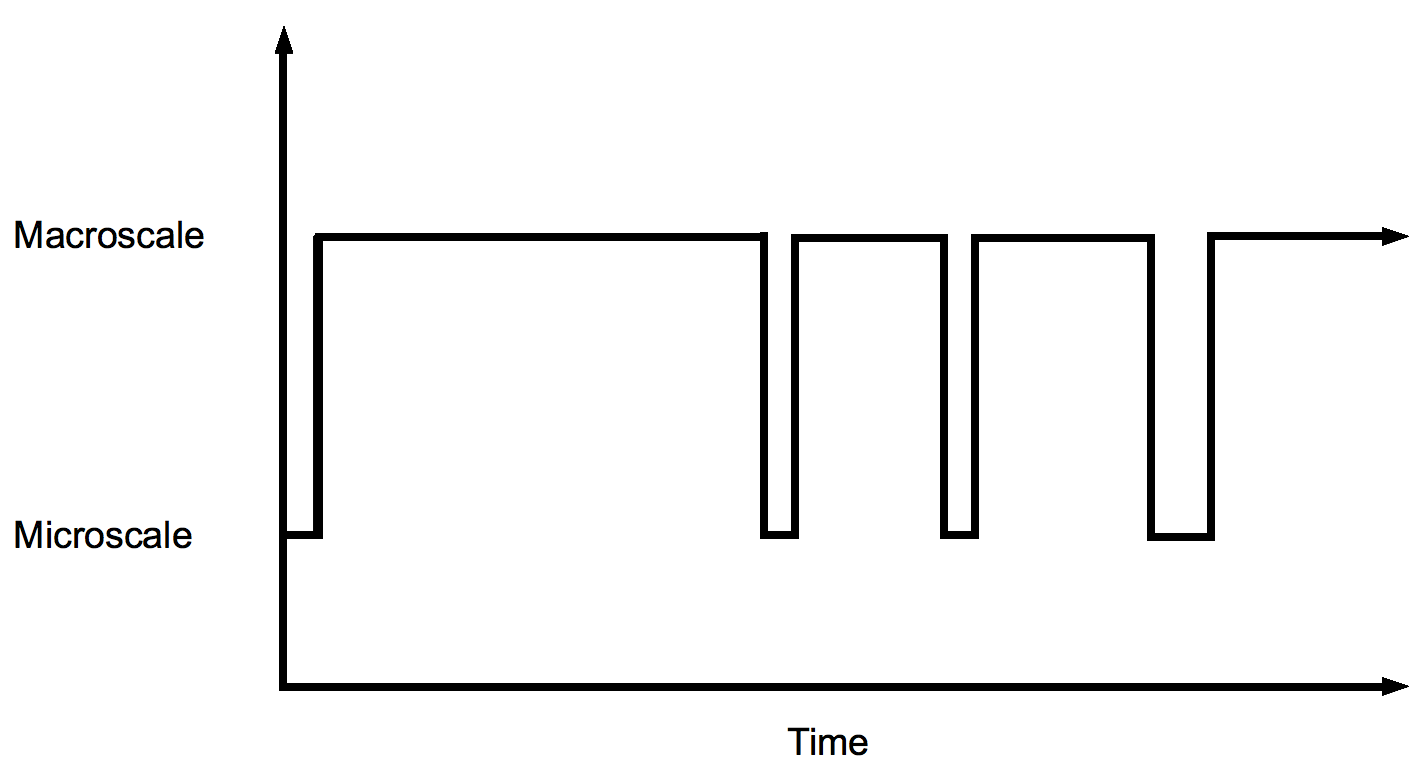
\includegraphics[height = 0.5\textheight]{scheme.png}
			\end{center}
	\end{frame}
	
	\begin{frame}{HMM Structure}
		\begin{itemize}
			\item  A \emph{compression} operator, $Q$, maps information from the microscale state to the macroscale
			\item  A \emph{reconstruction} operator, $R$, reconstructs the microscale model using the macroscale state
		\end{itemize}
		\begin{center}
			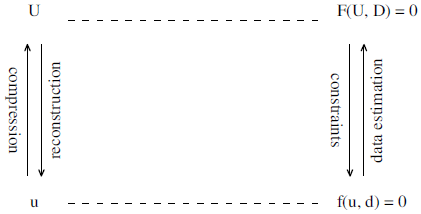
\includegraphics[width=0.7\textwidth]{framework.png}
			\\\tiny HMM Framework (Weinan E et al, 2006)
		\end{center}
	\end{frame}
	
	\begin{frame}{Types of Problems}
		\begin{enumerate}[leftmargin=1.75cm]
			\item[\textbf{Type A:}] Microscopic model is only required near isolated defects or singularities in the domain
			\vspace{1em}
			\item[\textbf{Type B:}] A nearly closed macroscale model exists but is not sufficiently explicit. The microscale model closes the system and provides missing information
			\vspace{1em}
			\item[\textbf{Type C:}] Problems with features of both \emph{Type A} and \emph{Type B} problems
			\vspace{1em}
			\item[\textbf{Type D:}] Problems that exhibit self-similarity
		\end{enumerate}
	\end{frame}
	
	\subsection{Examples}
	\begin{frame}[t]{Type A Example: Dealing with isolated defects}
		\begin{itemize}
			\item  Constitutive relations to compute flux in cells without defects\vspace{1em}
			\item  Use MD to compute flux in cells that contain defects
		\end{itemize}
		\begin{center}
			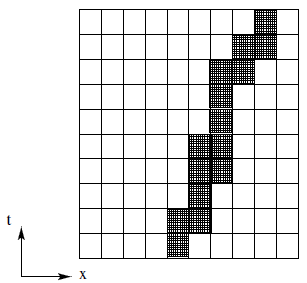
\includegraphics[width=0.5\textwidth]{typeA.png}
			\\\tiny Movement of defect over time (MD performed in black boxes). (Weinan E et al, 2006)
		\end{center}
	\end{frame}
	
	\begin{frame}[t]{Type B Example: Large-scale MD gas dynamics}
		\begin{itemize}
			\item  Finite volume solver on the macroscale\vspace{1em}
			\item  Constrained MD on cell boundaries to compute flux
		\end{itemize}
		\begin{center}
			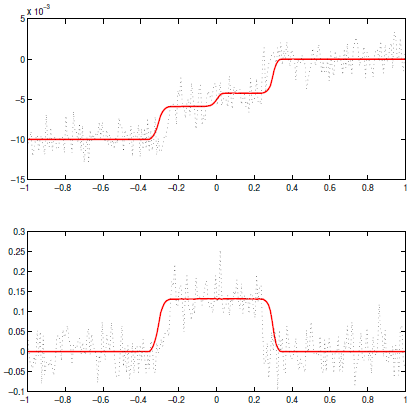
\includegraphics[height=0.65\textheight]{typeB.png}
			\\\tiny Computed strain (top) and velocity (bottom) compared with full MD simulation. (Weinan E et al, 2006)
		\end{center}
	\end{frame}
	
	\begin{frame}{HMM for Complex Fluids}
		\begin{itemize}
			\item Prototypical examples of HMM can be found in ``Heterogeneous multiscale method for the modeling of complex fluids and micro-fluidics'' by Weiqing Ren and Weinan E (2004)\vspace{1em}
			\item Macroscale: Continuum hydrodynamics\vspace{1em}
			\item Microscale: molecular dynamics\vspace{1em}
			\item They use the HMM methodology to simulate both Type A and Type B problems
		\end{itemize}
		
	\end{frame}
	
	\begin{frame}{HMM for Complex Fluids}
		\begin{columns}[T]
			\begin{column}{0.5\textwidth}
				\begin{itemize}
					\vspace{-0.5em}
					\item Type A: Contact surface between two immiscible fluids in a solid pipe\vspace{5em}
					\item Type B: Viscous stress tensor computed with MD at the boundary of the pipe using the Irving-Kirkwood formula, then extended throughout the domain with a constitutive relation
				\end{itemize}
			\end{column}
			\begin{column}{0.6\textwidth}
				\vspace{-0.5em}
				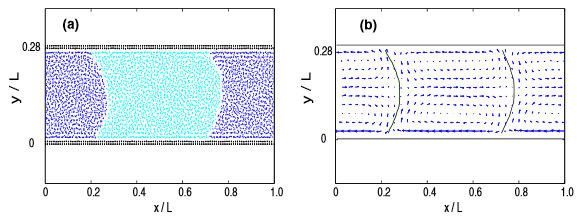
\includegraphics[width=1\textwidth]{weinan1.png}
				\\\tiny (a) Snapshot of all particle positions. (b) Averaged Velocity field and fluid-fluid interfaces. (Ren W and Weinan E, 2004)\\
				\vspace{0.25em}\hspace{1.1cm}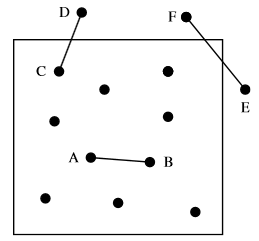
\includegraphics[width=0.7\textwidth]{weinan2.png}
				\\\tiny Computing average stress: particles outside the box also contribute. (Weinan E, 2011)\\
			\end{column}
		\end{columns}
	\end{frame}
	
	\section{HMM for Plasma Modeling}
	\subsection{Problem Statement}
	\begin{frame}{Our Goal}
		\begin{itemize}
			\item  Develop a proof-of-concept computational framework to model plasmas using HMM\vspace{1em}
			\begin{itemize}
				\item  We are not trying to model a specific problem\vspace{1em}				\item  We are trying to develop the framework to solve problems using this combination of models\vspace{1em}
			\end{itemize}
			\item  Macroscopic model: Kinetic theory using the BGK approximation of the Boltzmann equation (BGK)\vspace{1em}
			\item  Microscopic model: Molecular dynamics (MD)
		\end{itemize}
	\end{frame}
	
	\begin{frame}{Problem Statement}
		\begin{itemize}
			\item  Ions live in a two-dimensional periodic domain and are initialized such that their distribution is $x$-dependent, but uniform in $y$
			\vspace{0.5em}
			\begin{itemize}
				\item Use data from a 2D-2V MD microscale simulation to increase the accuracy of a 1D-2V BGK macroscale distribution function
				\vspace{0.5em}
				\item  May have $n$ species with different masses and charges
				\vspace{0.5em}
			\end{itemize}
			\vspace{0.5em}
			\item  The mathematical framework is built up from first principles and designed to be as general as possible
			\vspace{0.5em}
			\item  \emph{Type B} problem: we are using the MD to close our macroscale kinetic model
		\end{itemize}
	\end{frame}
	
	\subsection{Model Formulation}
	\begin{frame}{Model Choices}
		\begin{center}
			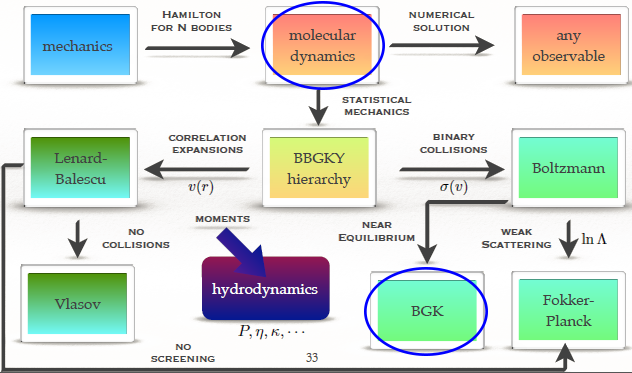
\includegraphics[width=1\textwidth]{KT_structure.png}
			\\\tiny Structure of kinetic theory models (Murillo, 2015)
		\end{center}
		
	\end{frame}
	
	%\begin{frame}{Model Formulation}
%		\begin{itemize}
%			\item  The models are derived from a Klimontovich distribution of $N$ particles, $\phi_k$, that stores the location, $\mathbf{r}_i$, and velocity, $\mathbf{v}_i$, of each ion $i$ of each species $k$ at a given time $t$:
%			\begin{equation*}
%				\phi_k(\mathbf{r},\mathbf{v},\{\mathbf{r}_\alpha\}_{\alpha=1}^{N},\{\mathbf{v}_\alpha\}_{\alpha=1}^{N},t) = \sum_{i\in S_k}\delta\left(\mathbf{r}-\mathbf{r}_i(t)\right)\delta\left(\mathbf{v}-\mathbf{v}_i(t)\right).
%			\end{equation*}
%			\vspace{0.5em}
%			\item  To preserve generality, we formulate our equations in a dimensionless form using a set of plasma parameters and arbitrary reference density $n_0$, temperature $T_0$, and mass $m_0$
%		\end{itemize}
%	\end{frame}
	
	
	
	\begin{frame}[t]{Microscale MD Model}
		\vspace{1em}
		\begin{itemize}
			\begin{columns}
				\begin{column}{0.9\textwidth}
					\item  2D-2V molecular dynamics with periodic boundary conditions
				\end{column}
				\begin{column}{0.0\textwidth}\end{column}
			\end{columns}
			\vspace{-1.5em}
			\begin{columns}
				\begin{column}{0.5\textwidth}
					\item  Solving a system of simple ODEs:
					\begin{align*}
					\dot{\boldsymbol{x}} &= \boldsymbol{v}	&	\dot{\boldsymbol{v}} &= \frac{\boldsymbol{F}}{m}
					\end{align*}
					\item  Particles interact through the Yukawa potential
					\vspace{0.5em}
					\item  Nearest neighbor lists with cutoff radius for $O(N)$ performance
				\end{column}
				\begin{column}{0.4\textwidth}
					\vspace{1em}
					\begin{center}
						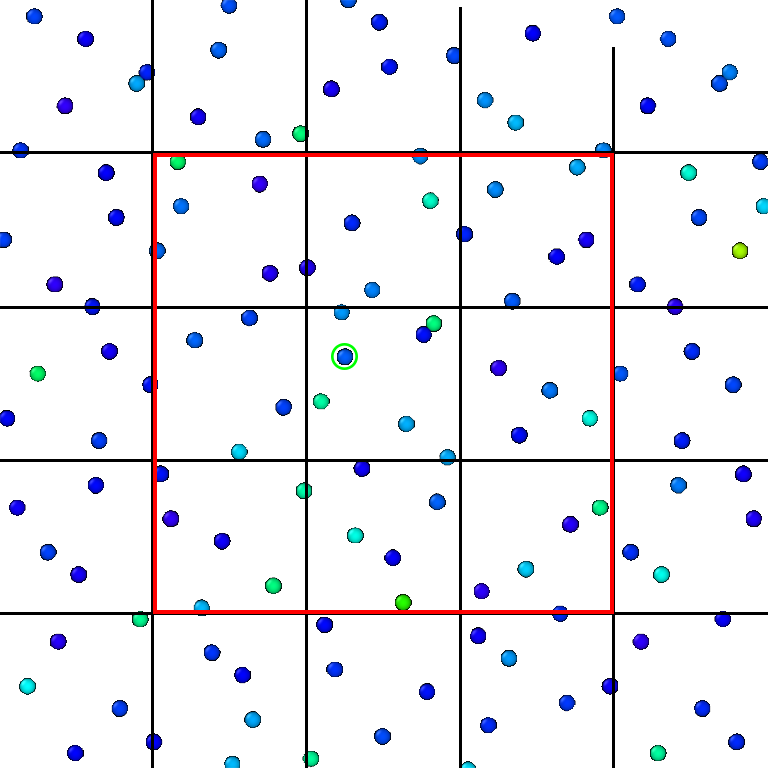
\includegraphics[height=0.5\textheight]{MD_diagram.png}
						\\\tiny MD snapshot with nearest neighbor cells
					\end{center}
				\end{column}
			\end{columns}
		\end{itemize}
	\end{frame}
	
	\begin{frame}{MD Implementation}
		\begin{itemize}
			\item  Velocity Verlet time evolution:\vspace{-0.2em}
			\small\begin{align*}
			v\left(t+\frac{\Delta t}{2}\right) &= v(t) + \frac{\Delta t}{2}\frac{F(t)}{m} \\
			x(t+\Delta t) &= x(t) + \Delta t\:v\left(t+\frac{\Delta t}{2}\right) \\
			v(t+\Delta t) &= v\left(t+\frac{\Delta t}{2}\right) + \frac{\Delta t}{2}\frac{F(t+\Delta t)}{m}
			\end{align*}\normalsize
			\item  Yukawa potential for particles $i$, $j$:\vspace{-0.2em}
			\small\begin{align*}
			V_{ij} &= \frac{Z_iZ_je^2}{4\pi\varepsilon_0r_{ij}}e^{-\frac{r_{ij}}{\lambda}} \\
			F_{ij} &= -\frac{\partial V_{ij}}{\partial r_{ij}} = V_{ij}\left(\frac{1}{r_{ij}}+\frac{1}{\lambda}\right)
			\end{align*}\normalsize
			\item  Track energy to ensure total energy is conserved
		\end{itemize}
	\let\thefootnote\relax\footnotetext{\tiny Thank you to Mathieu Marciante for the base MD code.}
	\end{frame}
	
	\begin{frame}{Deriving BGK from MD}
		\begin{itemize}
			\item  We construct a Klimontovich distribution, $N_k$, for each species that encodes the location, $\mathbf{r}_i$, and velocity, $\mathbf{v}_i$, of each ion $i$ of each species $k$ at a given time $t$:
			\begin{equation*}
				N_k(\mathbf{r},\mathbf{v},\{\mathbf{r}_\alpha\}_{\alpha=1}^{N},\{\mathbf{v}_\alpha\}_{\alpha=1}^{N},t) = \sum_{i\in S_k}\delta\left(\mathbf{r}-\mathbf{r}_i(t)\right)\delta\left(\mathbf{v}-\mathbf{v}_i(t)\right).
			\end{equation*}
			\item After defining the distribution of species $k$ as 
			\[f_1^{(k)}(\mathbf{r},\mathbf{v},t)=E[N_k],\]
			we use the Hamiltonian of the system of all species to derive a partial differential equation for $f_1^{(k)}$
		\end{itemize}
	\end{frame}
	
		\begin{frame}{Model Derivation}
		\begin{itemize}
			\item  For a general potential energy $U_{\{kl\}}$ that depends on the species of the two ions as well as their positions, this can be written as
			\begin{align*}
			\frac{\partial f_1^{(k)}}{\partial t}=&-\mathbf{v}\cdot\nabla_\mathbf{r}f_1^{(k)}\\&+\frac{1}{m_k}\nabla_\mathbf{r}\cdot\nabla_\mathbf{v}\left(\sum_l\int U_{\{kl\}}(\mathbf{r},\mathbf{r}')f_{2}^{(kl)}(\mathbf{r},\mathbf{v},\mathbf{r}',\mathbf{v}',t)\,d\mathbf{r}'\right)
			\end{align*}
			\item This defines the BBGKY hierarchy, which is still exact		
			\vspace{0.25em}
		\end{itemize}
		\begin{center}
			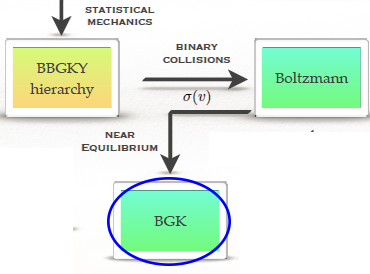
\includegraphics[height=0.3\textwidth]{KT_structure_zoom.png}
		\end{center}
	\end{frame}
	
	\begin{frame}{Model Derivation}
	\begin{itemize}
	\item The $f_2^{(kl)}$ are eight dimensional plus time, and so are very difficult to capture with a small MD simulation
	\vspace{1em}
	\begin{itemize}
	\item Instead, we use the BGK approximation:
	\[f_2^{(kl)}(\mathbf{r},\mathbf{v},\mathbf{r}',\mathbf{v}',t)=f_1^{(k)}(\mathbf{r},\mathbf{v},t)f_1^{(l)}(\mathbf{r}',\mathbf{v}',t)+C
	\]
	\end{itemize}
	\item This results in:
			\begin{align*}
				\frac{\partial f_1^{(k)}}{\partial t}=&-\mathbf{v}\cdot\nabla_\mathbf{r}f_1^{(k)}\\&+\frac{1}{m_k}\nabla_\mathbf{r}\left(\sum_l\int U_{\{kl\}}(\mathbf{r},\mathbf{r}')n_l(\mathbf{r}',t)\,d\mathbf{r}'\right)\cdot\nabla_\mathbf{v}f_1^{(k)}\\&+\sum_l\frac{f_{eq}^{(kl)}-f_1^{(k)}}{\tau_{kl}}
			\end{align*}where $n_l(\mathbf{r}',t)=\int f_1^{(l)}d\mathbf{v}$ is the ion density of species $l$
			\end{itemize}
			\end{frame}
			
			\begin{frame}{Model Derivation}
			\begin{itemize}
	\item Let $U_{\{kl\}}$ be the Yukawa potential or the Coulomb potential, and $E(\mathbf{r},t)$ be the electric field at $\mathbf{r}$ at time $t$ due to this potential. Then, this reduces to the Vlasov equation:
			\begin{equation*}
			\frac{\partial f_1^{(k)}}{\partial t}+\mathbf{v}\cdot\nabla_\mathbf{r}f_1^{(k)}+\frac{Z_k e}{m_k}E(\mathbf{r},t)\cdot\nabla_\mathbf{v} f_1^{(k)}=\sum_l\frac{f_{eq}^{(kl)}-f_1^{(k)}}{\tau_{kl}}
			\end{equation*}
			
			\item We evolve the BGK simulation in only the $x$ direction, assuming uniformity in the $y$ direction\begin{equation*}
			\frac{\partial f_1^{(k)}}{\partial t}+v_x\frac{\partial f_1^{(k)}}{\partial x}+\frac{Z_k e}{m_k}E(x,t)\frac{\partial f_1^{(k)}}{\partial v_x}=\sum_l\frac{f_{eq}^{(kl)}-f_1^{(k)}}{\tau_{kl}}
			\end{equation*}
			\item If our 1D-2V macroscale simulation can capture the behavior of the 2D-2V microscale simulation, it will be a testament to the effectiveness of HMM
\end{itemize}
	\end{frame}
	
	\begin{frame}{Kinetic Implementation}
		\begin{itemize}
			\item  We use a second order finite volume method to evolve the PDE\end{itemize}\begin{center}
			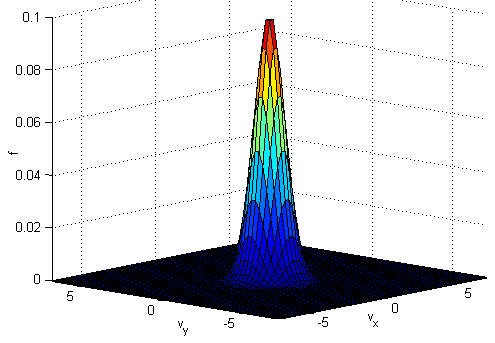
\includegraphics[height=0.3\textheight]{example_f.png}
			\\\tiny $f_1^{(k)}(\boldsymbol{v})$ at a single $x$ location
		\end{center}
			\begin{itemize}\item  The electric field, assuming a Yukawa potential, is computed by using the trapezoid rule to approximate the double integral:
			\begin{align*}E(x,t)=-\frac{e}{4\pi\epsilon_0}\int_{-\infty}^\infty\int_{-\infty}^\infty&\rho(x-x',t)\frac{e^{-|\mathbf{r}'|/\lambda}}{|\mathbf{r}'|}\cdot\\&\left(\frac{1}{|\mathbf{r}'|}+\frac{1}{\lambda}\right)\frac{x'}{|\mathbf{r}'|}\,dx'\,dy'
			\end{align*}

		\end{itemize}
	\let\thefootnote\relax\footnotetext{\tiny Thank you to Jeff Haack for the base KT code.}
	\end{frame}
	
	
	
	\begin{frame}[t]{Comparison of Models}
		\vspace{-0.8em}
		\begin{columns}
			\begin{column}{0.55\textwidth}
				\begin{center}\textbf{Molecular Dynamics}\end{center}\vspace{-0.8em}
				\begin{itemize}
					\item  \color{blue}Conserves total energy
					\item  Simulating random walk of particle interactions ``exactly''
					\item  Full particle correlations
					\item  \color{red}Noisy, need ensemble average to calculate bulk properties
					\item  Requires very small time step
					\item  \ovalbox{Computationally expensive}
				\end{itemize}
			\end{column}
			\begin{column}{0.55\textwidth}
				\begin{center}\textbf{Kinetic Theory}\end{center}\vspace{-0.8em}
				\begin{itemize}
					\item  \color{red}Only conserves kinetic energy
					\item  Simulating particle interactions in average sense
					\item  No particle correlation data
					\item  \color{blue}Can calculate bulk properties directly from $f$
					\item  Relatively large time steps
					\item  \ovalbox{Computationally inexpensive}
				\end{itemize}
			\end{column}
		\end{columns}
		\begin{center}
			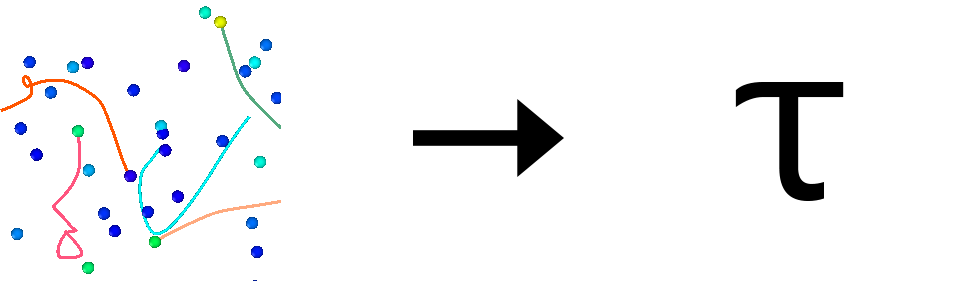
\includegraphics[height=0.3\textheight]{random_walk.png}
		\end{center}
	\end{frame}
	
	\subsection{Connecting the Models}
	\begin{frame}{Connecting the Models with $\tau$}
		\begin{itemize}
		\item BGK attempts to approximate the collisional terms of the Boltzmann equation by relaxing the distribution towards interparticle equilibria with relaxation times $\tau_{kl}$
		\vspace{1em}
		\item Boltzmann also has an $H$ theorem:
		\[H(t)=\int\int  f(\mathbf{r},\mathbf{v},t)\left[\log\left(f(\mathbf{r},\mathbf{v},t)\right)-1\right]\,d\mathbf{r}\,d\mathbf{v}
		\]\item The entropy $H$ is monotonically decreasing
		\vspace{1em}
		\item We choose $\tau_{kl}$ such that the observed rate of decrease of $H$ in the MD simulation matches the rate of decrease of $H$ in the BGK model
		\end{itemize}
	\end{frame}

	\begin{frame}{Connecting the Models with $\tau$}
		\begin{itemize}
		\item $H$ can be computed from our MD data by:
		\[H(t)=\log\left(\prod_iE\left[\sum_j\delta(\mathbf{r}_i-\mathbf{r}_j)\delta(\mathbf{v}_i-\mathbf{v}_j)\right]\right)-N
		\]\item The expected value can be computed as a time average, and the rate of change of $H$ can be computed by differentiating this time series
		\vspace{1em}
		\item $H'(t)$ in the BGK can be computed by using the PDE to simplify
		\[H'(t)=\int\int \frac{\partial f}{\partial t}\log(f)\,d\mathbf{r}\,d\mathbf{v}
		\]\item We plan to pair like terms to compute the relaxation times for each species pair
		\end{itemize}
	\end{frame}
	
	\subsection{Challenges}
	\begin{frame}{Challenges}
		\begin{itemize}
			\item[1. ]  How often do we need to update $\tau$?
			\item[2. ]  How long do we need to run the MD to recover $\tau$?
			\item[3. ]  How do we initialize the MD model from $f$?
			\item[4. ]  How do we return to the BGK model from MD?
		\end{itemize}
		\begin{center}
			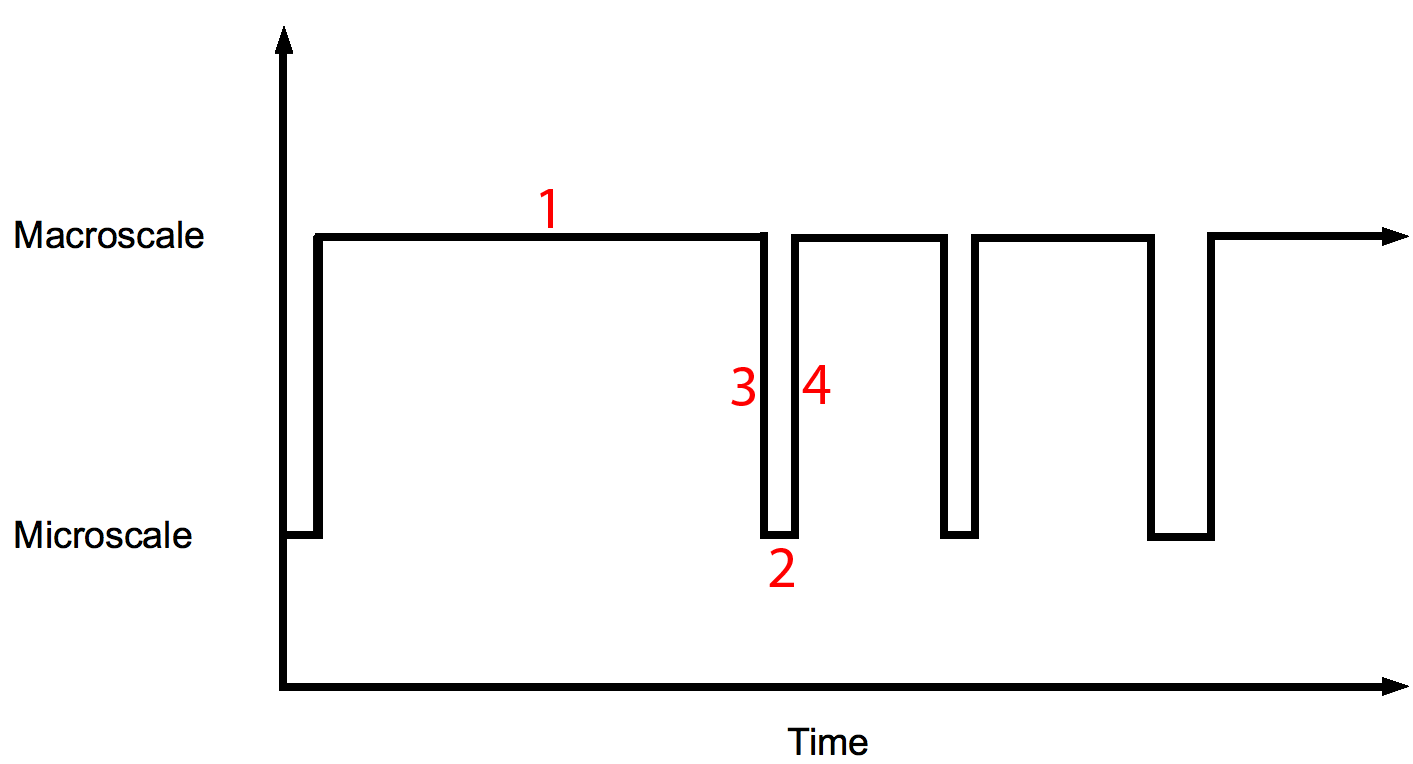
\includegraphics[height=0.55\textheight]{scheme2.png}
		\end{center}
	\end{frame}
	
	\begin{frame}{Reconstruction (How to initialize MD from $f$)}
		\begin{itemize}
		\item Because $f$ is high dimensional, directly sampling it accurately would require prohibitively many particles
		\vspace{0.5em}
		\item We have no knowledge of the particle correlations
		\vspace{0.5em}
		\item We use a three-step process for initializing MD
		\vspace{0.5em}
		\begin{itemize}
		\item[1. ] Use a Halton sequence to place a set number of particles in $x$ bins to match the density of $f$
		\vspace{0.5em}
		\item[2. ] Use a Langevin thermostat to equilibrate each bin to its proper temperature
		\vspace{0.5em}
		\item[3. ] Once properly correlated, draw new velocities for each particle from the velocity distribution at that $x$ position
		\end{itemize}
		\end{itemize}
	\end{frame}
	
	\begin{frame}{Reconstruction (Equilibration)}
		\begin{itemize}
			\item Uses Langevin dynamics, where $F_i$ is replaced by:
			\begin{equation*}
			F_i = \sum_{j}F_{ij} - m_i\gamma v_i + \sqrt{\frac{2\gamma m_iT}{\Delta t}}\eta
			\end{equation*}
			\item Particles are constrained to their bins with reflective boundary conditions in $x$ to preserve density
			\begin{itemize}
				\item They do interact with particles in other bins, ensuring that inter-bin correlations are captured
			\end{itemize}
		\end{itemize}
		\begin{center}
			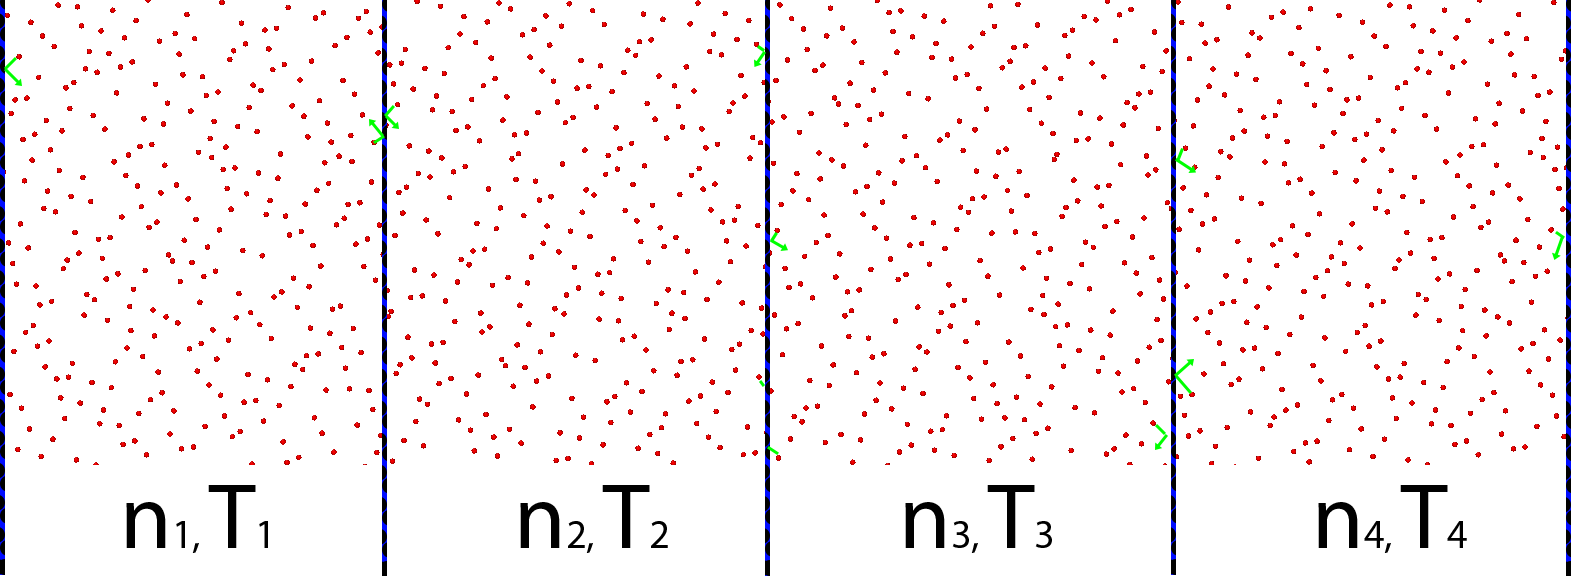
\includegraphics[width=0.9\textwidth]{figures/equilibration.png}
			\\\tiny Scheme for equilibration phase.
		\end{center}
	\end{frame}
	
	\begin{frame}{Sidebar: why we don't equilibrate first moment}
		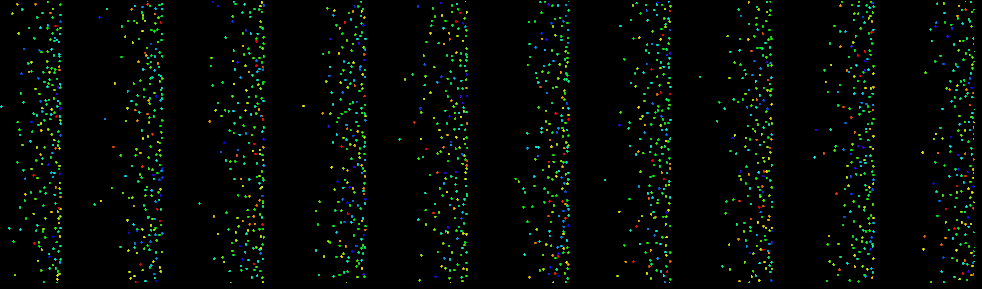
\includegraphics[width=1.0\textwidth]{figures/shitty_equilibration.png}
	\end{frame}
	
	\begin{frame}{Reconstruction (Velocity Resample)}
		\begin{itemize}
			\item Interpolate the velocity distribution for each bin so it is not ``too discrete''
			\vspace{1em}
			\item Assign particle velocities to particles in each bin by sampling the 2D probability distribution function
			\vspace{1em}
			\item Our velocity resampling algorithm accurately captures at least the first three moments of the velocity distribution with sufficient particles
			\vspace{1em}
			\item \emph{Question}: How important are the velocity correlations that we are throwing out?
		\end{itemize}
	\end{frame}
	
	\begin{frame}{Compression (How to go back to BGK from MD)}
		\begin{itemize}
		\item We have two options when returning to BGK from MD:
		\vspace{0.5em}
		\begin{itemize}
		\item $f$ is defined as $E[\sum_{i}\delta(\mathbf{r}-\mathbf{r}_i)\delta(\mathbf{v}-\mathbf{v}_i)]$
		\vspace{0.5em}
		\begin{itemize}
		\item When we compute $\tau_{kl}$ using time averages, we can also compute this expected value and reinitialize $f$ at the end time of MD\vspace{0.5em}
		\end{itemize}
		\item We can ``pause'' the kinetic distribution, use MD to compute new $\tau_{kl}$ values, and then ``restart'' the BGK simulation where we left off\vspace{0.5em}
		\end{itemize}
		\item The first option is more accurate, but is subject to additional statistical noise that the second option avoids
		\end{itemize}
	\end{frame}
	
%	\subsection{Results}
%	\begin{frame}{Where are we now?}
%		\begin{itemize}
%		\item 
%		\end{itemize}
%	\end{frame}
	
	\subsection{Preliminary Results}
	\begin{frame}{Preliminary Results}
		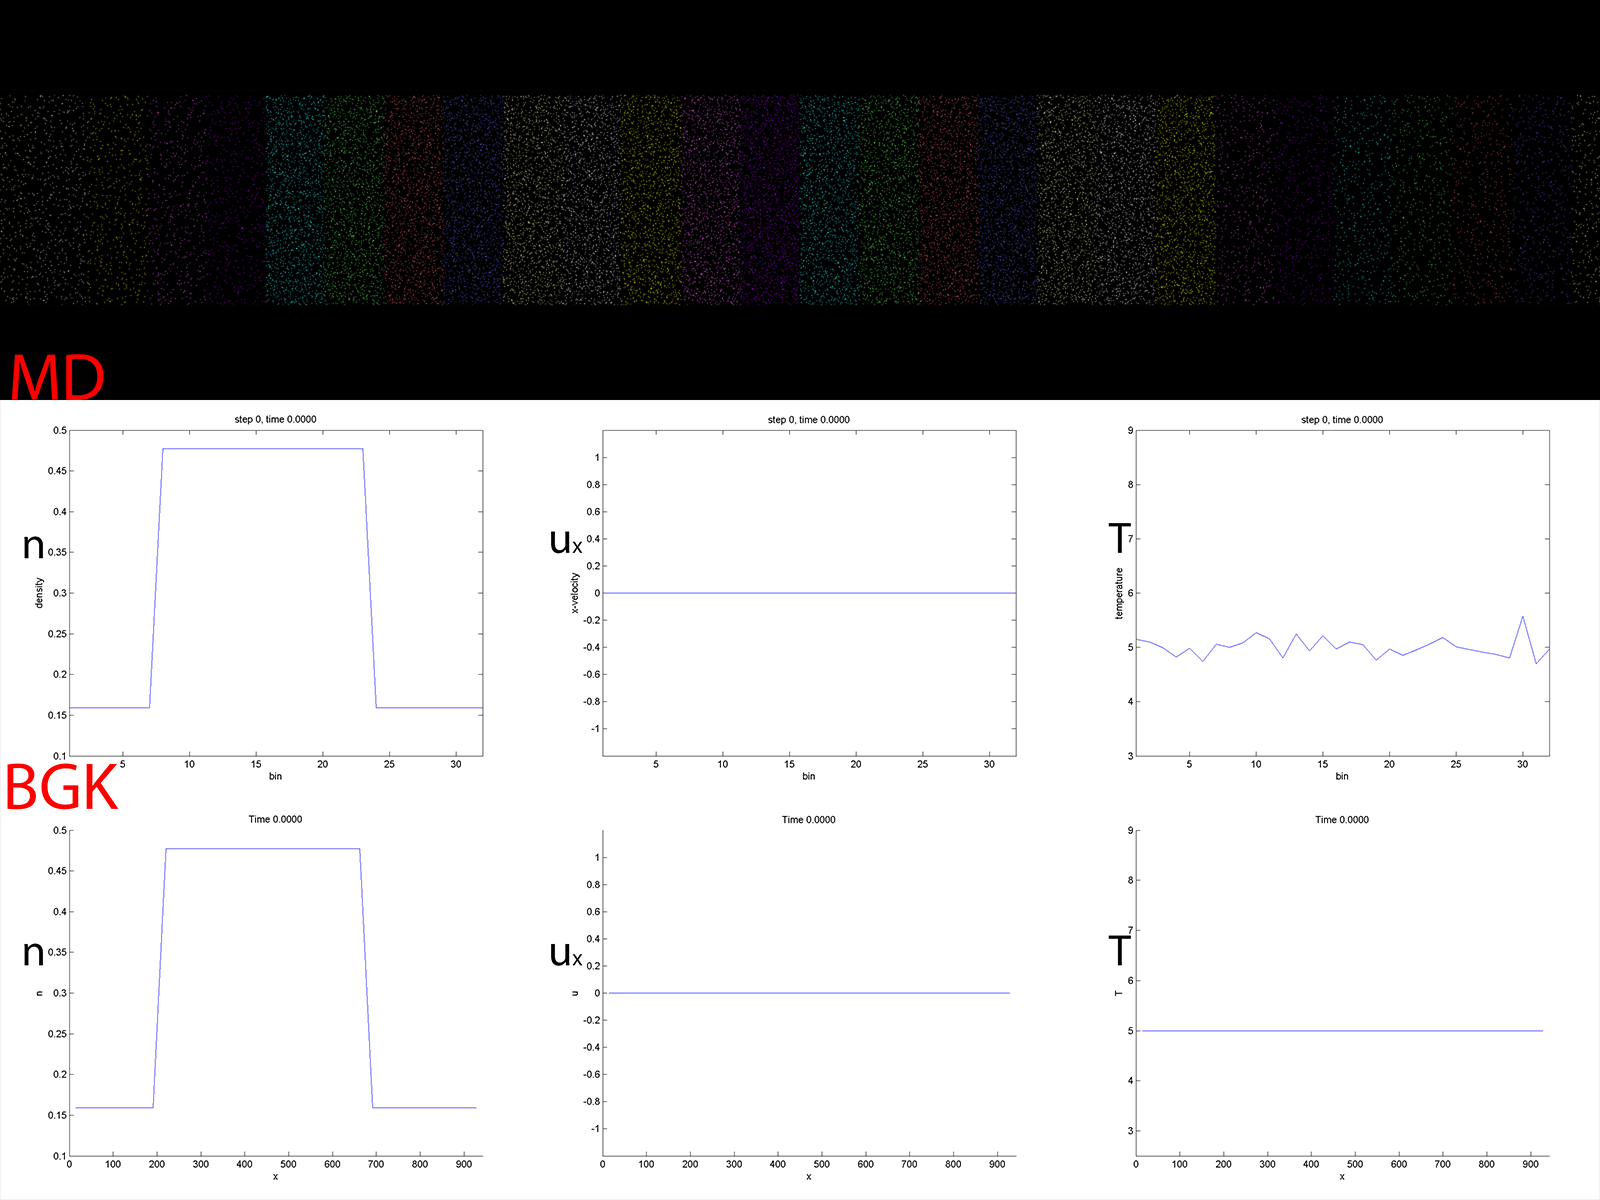
\includegraphics[width=1.0\textwidth]{BGK_MD_movie0000.png}
	\end{frame}
	
	\section{Future Work}
	\begin{frame}{Short Term Future Work}
		\begin{itemize}
			\item Implement connection between the KT and MD models and compare results to full MD simulation
			\vspace{0.5em}
			\item Consider alternate ways to compute $\tau_{kl}$
			\vspace{0.5em}
			\item More exploration of MD initialization:
			\vspace{0.5em}
			\begin{itemize}
				\item When are velocity correlations important?
				\vspace{0.5em}
				\item How many particles do we need to accurately capture $f$?
			\end{itemize}
			\vspace{0.5em}
			\item Adaptive MD time step to avoid energy spikes when two particles get too close
		\end{itemize}
	\end{frame}
	
	\begin{frame}{Long Term Future Work}
		\begin{itemize}
			\item Implement the model outside Matlab to solve larger problems
			\vspace{1em}
			\item Implement in full three dimensions in both regimes
			\vspace{1em}
			\item Test model with multi-species scenarios
			\vspace{1em}
			\item Use a different kinetic model (e.g. BBGKY)
			\vspace{1em}
			\item Use other interaction potentials to solve different problems			
			
		\end{itemize}
	\end{frame}
	
	\section{Summary}
	\begin{frame}{Summary}
		\begin{itemize}
			\item HMM provides a framework to provide hybrid multiphysics simulations that combine the accuracy of the microscale with the efficiency of the macroscale
			\vspace{1em}
			\item Extra attention must be paid to the connection between the two models (compression and reconstruction)
			\vspace{1em}
			\item We have the theoretical framework to model plasmas using kinetic theory and molecular dynamics
			\vspace{1em}
			\item The ``connective tissue'' is not fully there yet: we have some ideas and would love your input!
		\end{itemize}
	\end{frame}
	
	\section{Acknowledgements}
	\begin{frame}{Acknowledgements}
		We would like to extend our thanks to the following individuals and organizations:\vspace{1em}
		\begin{itemize}
		\item The Los Alamos National Lab Computational Physics Student Summer Workshop for providing a stimulating work environment, and funding our summer research\vspace{1em}
		\item Jeff Haack and Mathieu Marciante for providing the separate BGK and MD codes we used as a starting point\vspace{1em}
		\item Jeff Haack and Michael Murillo for many helpful conversations and overlong meetings
		\end{itemize}
	\end{frame}
	
	\section{References}
	\begin{frame}[allowframebreaks]{References}
	\nocite{weinan2007heterogeneous,weinan2011principles,klimontovich1983kinetic,ren2005heterogeneous,franklin2000boltzmann,hadjiconstantinou1997heterogeneous,flekkoy2000hybrid,nie2004continuum,li1999nearly}
		\bibliography{../../FinalPaper/HMM_bib}
	\end{frame}
	
	\section{Mathematical Details}
	
	
	\begin{frame}{Mathematical Details}
		\begin{itemize}
			\item  The ion-circle radius defines the length scale
			\begin{equation*}
			a = \frac{1}{\sqrt{\pi n}}
			\end{equation*}
			\item  The plasma frequency defines the (inverse) time scale
			\begin{equation*}
			\omega_p = \sqrt{\frac{Z^2e^2n}{2\varepsilon_0am}}
			\end{equation*}
			\item  The dimensionless coupling parameter of the plasma defines the ratio of potential energy to kinetic energy
			\begin{equation*}
			\Gamma = \frac{Z^2e^2}{4\pi\varepsilon_0aT}
			\end{equation*}
			\item  The screening parameter is the dimensionless screening length
			\begin{equation*}
			\kappa = \frac{a}{\lambda}
			\end{equation*}
		\end{itemize}
	\end{frame}
	
	\begin{frame}{Mathematical details}
		\begin{itemize}
			\item  To preserve generality, we formulate our equations in a dimensionless form using a set of plasma parameters and arbitrary reference density $n_0$, temperature $T_0$, and mass $m_0$
			\vspace{1em}
			\begin{itemize}
			\item $\Gamma$ is selected so we are in a kinetically relevant regime
			\end{itemize}
		\end{itemize}
	\end{frame}
	
\end{document}